\textbf{\normalsize More General Regularization Terms and \hyperref{https://en.wikipedia.org/wiki/Inpainting}{}{}{Image Inpainting}}

~\\
{\color{navy}
	\textbf{Background:}\\
	Based on the idea of Tikhonov regularization we can use more general regularization terms by transforming the vector $x$ with some matrix $G\in\Rmn$. Specifically, let us consider the more general regularized problem
	\begin{equation} \label{prob:regularized_leastsquares}
	\min_{x\in \Rn} \|Ax-b\|_2^2 + \frac{\delta}{2}\|Gx\|_2^2,~~~\delta > 0 ~\text{small}.
	\end{equation}
	The corresponding ``regularized'' normal equation then reads as 
	\begin{equation}\label{eq:regularized_normaleq}
	(A^TA  + \delta G^\top G)x = A^Tb. 
	\end{equation}
	Observe that for $G = I$ we obtain the standard Tikhonov (or $L^2$-) regularization. We easily see that if $G^\top G$ is positive definite, then so is $A^TA  + \delta G^\top G$ for positive $\delta$, so that \eqref{eq:regularized_normaleq} is uniquely solvable.\\~\\ 
	We will apply this framework to the problem of \hyperref{https://en.wikipedia.org/wiki/Inpainting}{}{}{image inpainting}. Therefore assume you are given the deteriorated image $b$, which is obtained from the \underline{unknown} original image $x$ through the following masking operation
	\begin{equation} \label{eq:masking_operation}
		b_i = \begin{cases}
		x_i & i \in \texttt{indices},\\
		0 & \text{else},
		\end{cases}
	\end{equation}
	where \texttt{indices} is a list of random pixels. In words, the pixels in \texttt{indices} survived, the rest is set to zero and therefore lost. We want to recover those lost pixels. Note that the images are considered being flattened and thus vectors, so that the masking operation \eqref{eq:masking_operation} can be written as a matrix-vector product
	$$b = Ax $$
	for some quadratic matrix $A$. You will see below that $A$ is not of full rank, so that we cannot simply solve this equation. Instead, we will seek for solutions of the regularized least squares problem \eqref{prob:regularized_leastsquares} by solving the linear equation \eqref{eq:regularized_normaleq}. 
	~\\
	For this purpose will stick to a particular $G$ which is related to what is called Sobolev (or $H^1$-) regularization. Specifically we consider the 1-d finite difference quotient
	\begin{equation}\label{eq:G}
	 G = \begin{pmatrix}
	  1 & &  &  \\
	  -1 & 1 &   &\\
	   &\ddots&\ddots & \\
	   & &-1 & 1\\
	 \end{pmatrix} \in \R^{(n+1)\times n},
	\end{equation}
	which has $1$ on the main diagonal, $-1$ on the first lower off-diagonal, $0$ everywhere else and is of dimension $(n+1)\times n$. Then, given the measured image $b$, the masking operator $A$ (we assume that we know which pixels are original) and the regularization $G$ we reconstruct the unknown image $x$ by solving equation \eqref{eq:regularized_normaleq}. See Figure below for an example experiment.
}
\begin{center}
	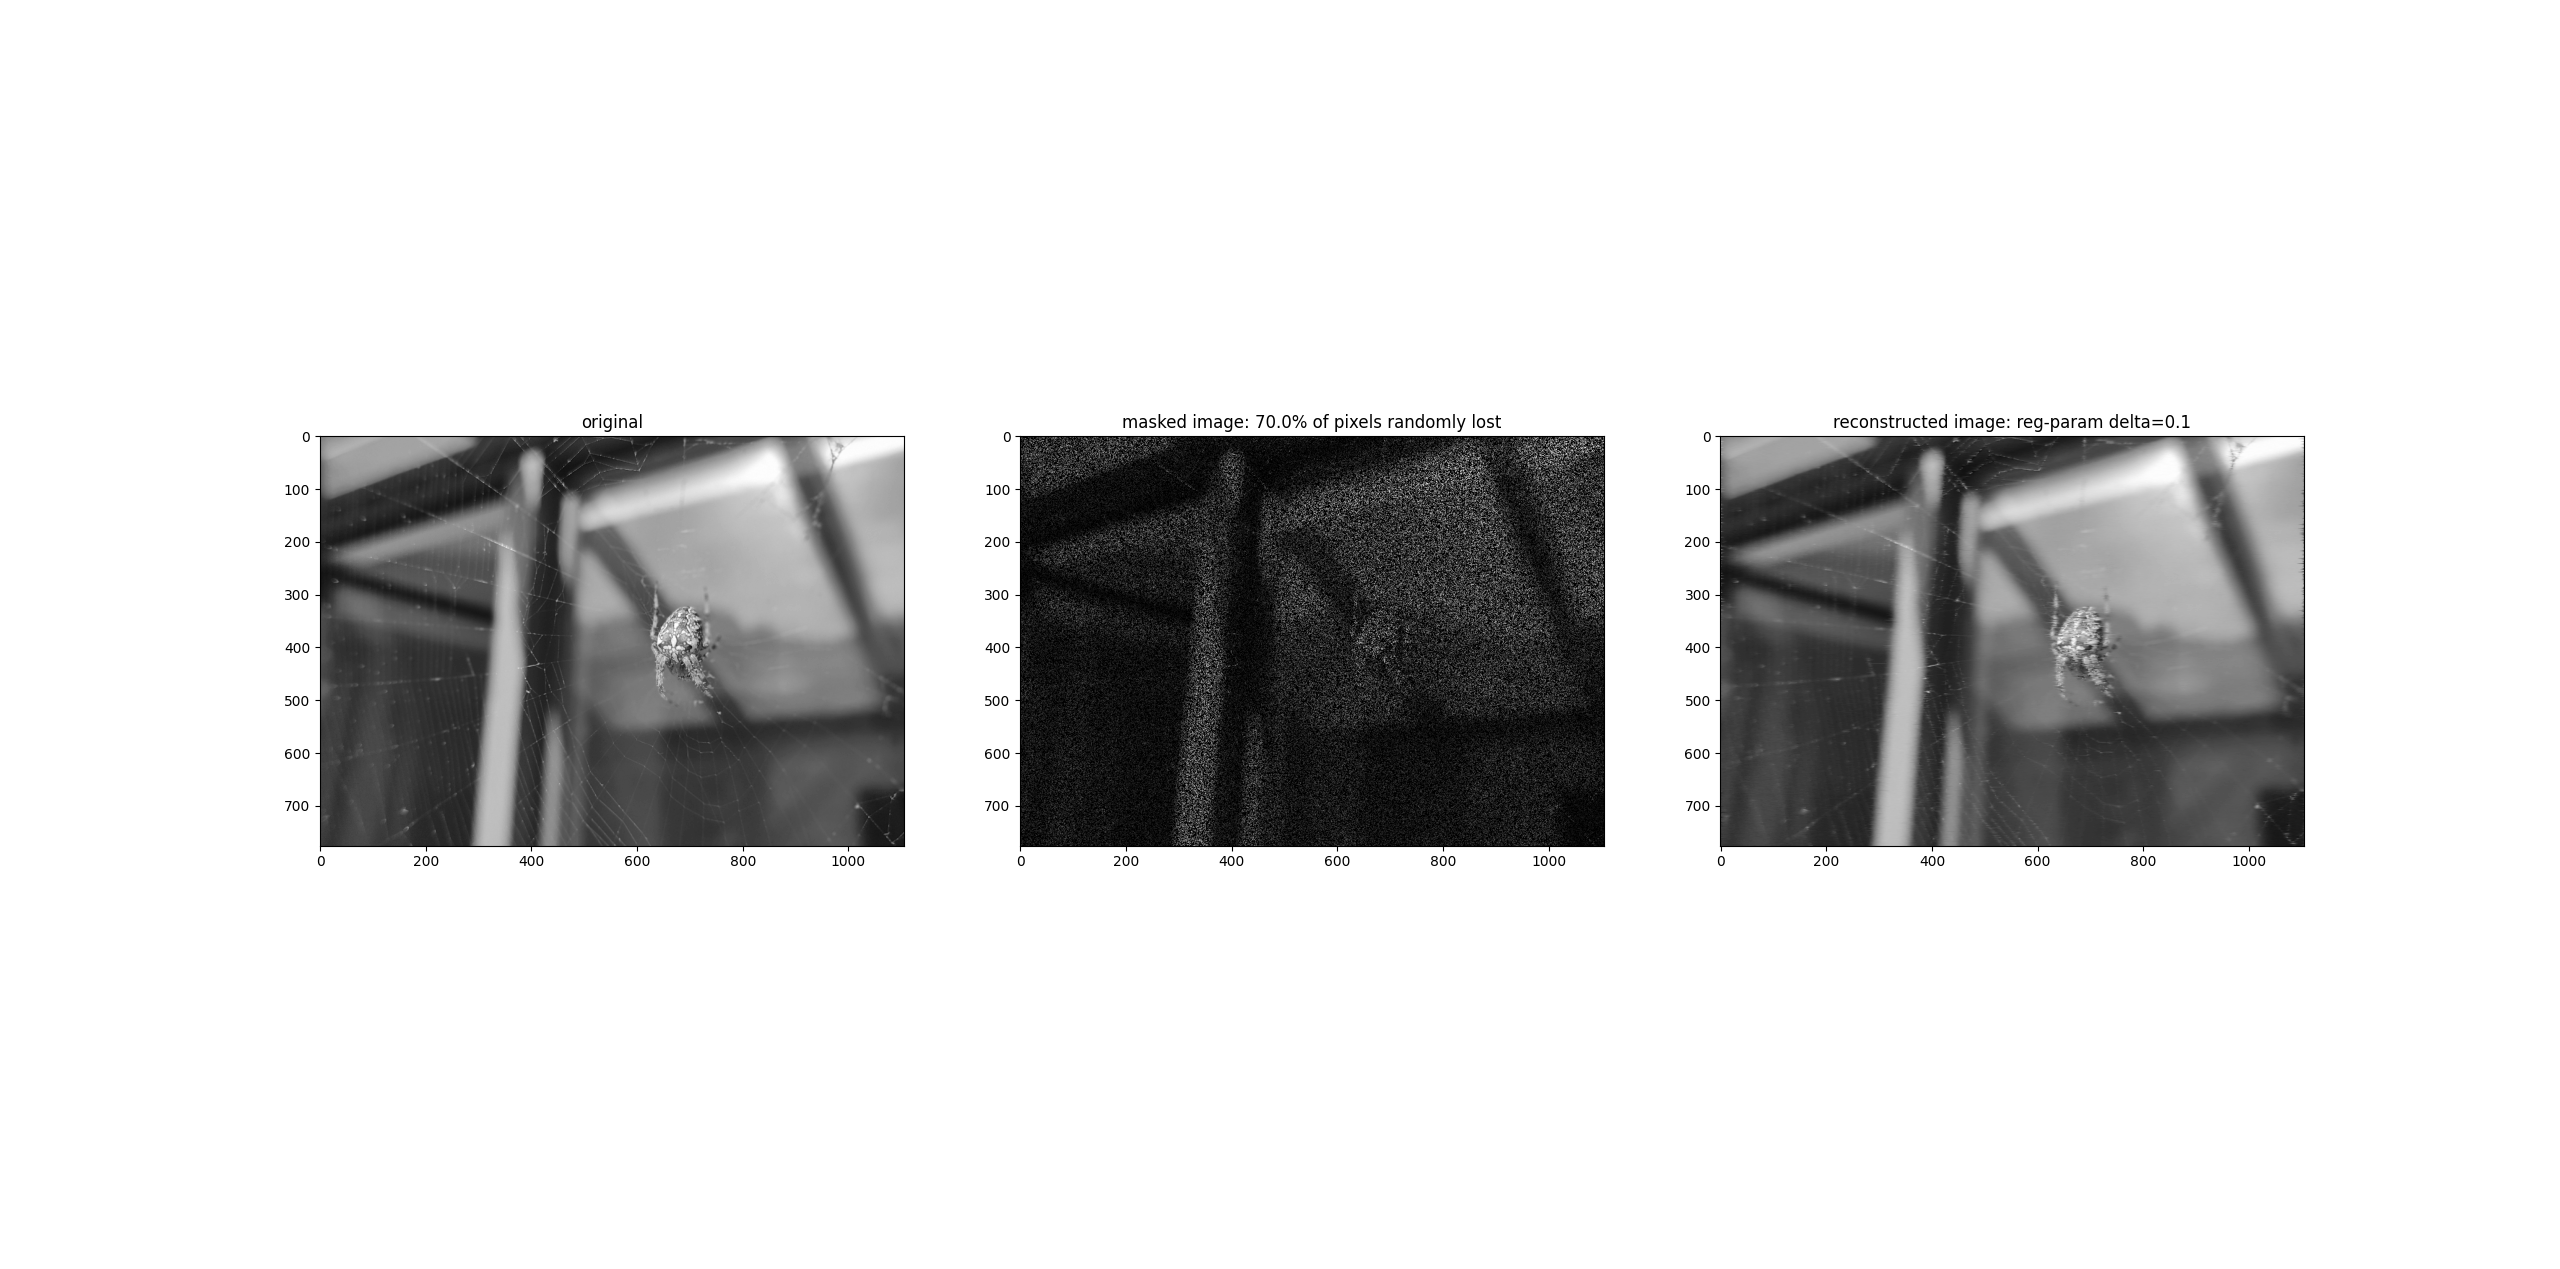
\includegraphics[trim={7cm 10.2cm 7cm 10.2cm},clip, width=1.\textwidth]{Image_Inpainting}\\~\\
	\textit{Example experiment.}
\end{center}
\newpage
\textbf{Step by Step}\\
First note that due to the high dimensional image data you need to work with sparse matrices (\texttt{scipy.sparse}); specifically you should work with the CSR format.
\begin{enumerate}
	\item \textbf{Choose original image:} Choose an image and load it in gray-scale as $H\times W$ \texttt{numpy.ndarray} using the code snippet:
	\lstinputlisting[firstline =7,lastline=13]{solution.py}
	\item \textbf{Masking:} Write a function 
	$$\texttt{b, indices = masking(img, percentage)},$$
	which takes as input an image \texttt{img} as $H\times W$ \texttt{numpy.ndarray} and a number \texttt{percentage} $\in (0,1)$ which indicates the percentage of pixels that are randomly kept. It shall return the masked image $b$ as an $n:=(H\cdot W)$-dimensional vector and the list \texttt{indices} $\subset \{0,\ldots, n-1\}$ indicating which pixels are original.
	\begin{itemize}
		\item Ultimately, the image needs to become a vector. For this purpose you can use for example the method \texttt{.ravel()}. No matter which method/function you choose, be aware of how the vector is flattened (standard is often: row-major/C-style order).
		\item To generate a random set of indices based on the parameter \texttt{percentage} have a look at the function \texttt{numpy.random.choice}.
	\end{itemize}
	\item \textbf{Solving:} Write a function 
	 $$\texttt{reconImg = inpainting(b, indices, delta, G)},$$
	 which expects a deteriorated image $b$ as vector of length $n$, a list \texttt{indices} $\subset \{0,\ldots, n-1\}$ of length $\leq n$ indicating which pixels are original, a regularization parameter \texttt{delta} $>0$ and a matrix \texttt{G} $\in \R^{m\times n}$. It then solves \eqref{eq:regularized_normaleq} and returns the solution as an $n$-dimensional vector \texttt{reconImg}.
	 \begin{itemize}
	 	\item The sparse  $(n \times n)$ masking matrix $A$ is zero everywhere except for $a_{ii} = 1$ for $i \in$\texttt{indices}. For example, you can easily implement this matrix with  \texttt{sparse.coo\_matrix} and then transform it to CSR format via its method \texttt{.tocsr()}.
	 	\item You can implement the sparse matrix $G$ from \eqref{eq:G} with the help of the function \texttt{scipy.sparse.eye}.
	 	\item You can then solve the system \eqref{eq:regularized_normaleq} with \texttt{scipy.sparse.linalg.spsolve}.
	 \end{itemize}
 	\item \textbf{Analysis:} 
 	\begin{itemize}
 		\item Play around with different choices for the parameters \texttt{delta} and \texttt{percentage}.
 		\item You can plot your images (original, masked, reconstructed) with $$\texttt{matplotlib.pyplot.imshow((...).reshape(H,W), cmap='gray')}.$$
 		\item Bonus: Try to recover the image with standard Tikhonov regularization, i.e., $G=I$. Do you have an idea why this does not work here?
 		\item Bonus: With this choice of $G$, you get flattening artifacts in one dimension (horizontal or vertical depending on your flattening approach) and at the boundary of the reconstructed image. Do you have an idea why? 
 	\end{itemize}
 \item \textbf{Bonus:} Instead of removing randomized set of pixels, remove a patch of the image. Can you reconstruct it?
\end{enumerate}


